\documentclass[tikz,border=2pt]{standalone}
\usepackage{amsmath,amssymb}
\usepackage{pgfplots}
\pgfplotsset{compat=1.18}
\usetikzlibrary{arrows.meta}
\begin{document}
% Expected value principle Pi(X) = (1+theta) E[X] with theta = 0.2: E[X] = 100 gives 120 (loading 20);
% adding a certain 10 moves E[X] to 110 and the premium to 132, not 120 + 10 = 130.
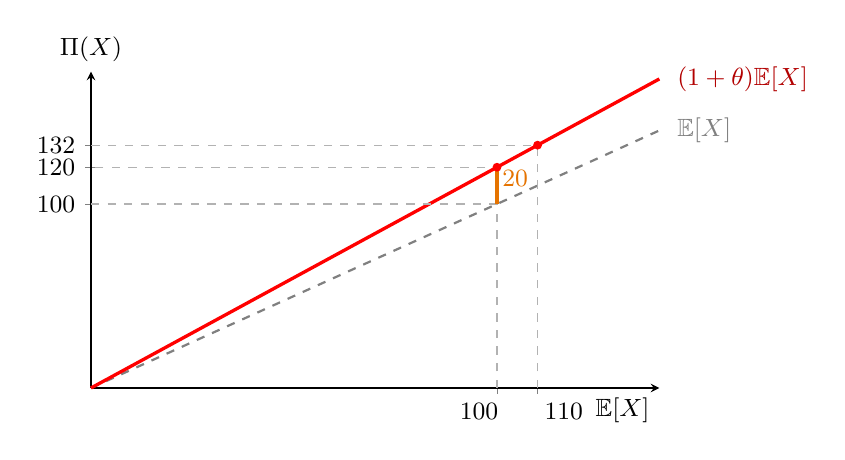
\begin{tikzpicture}[font=\small, >={Latex[length=2mm]}]
  \begin{axis}[
    axis lines=left, xmin=0, xmax=140, ymin=0, ymax=172,
    xtick={100,110}, xticklabels={,}, ytick={100,120,132},
    xlabel={$\mathbb E[X]$}, ylabel={$\Pi(X)$},
    xlabel style={at={(axis description cs:1,0)}, anchor=north east},
    ylabel style={rotate=-90, at={(axis description cs:0,1)}, anchor=south},
    width=8.8cm, height=5.6cm, clip=false
    ]
    \addplot[gray, thick, dashed, domain=0:140, samples=2] {x};
    \addplot[red, very thick, domain=0:140, samples=2] {1.2*x};
    \draw[gray!60, thin, dashed] (axis cs:100,0) -- (axis cs:100,120) -- (axis cs:0,120);
    \draw[gray!60, thin, dashed] (axis cs:110,0) -- (axis cs:110,132) -- (axis cs:0,132);
    \draw[gray!60, thin, dashed] (axis cs:0,100) -- (axis cs:100,100);
    \draw[orange!90!black, very thick] (axis cs:100,100) -- (axis cs:100,120);
    \node[orange!90!black, anchor=west, inner sep=1pt] at (axis cs:100.5,114) {$20$};
    \node[anchor=north east, xshift=4pt, yshift=-2pt] at (axis cs:100,0) {$100$};
    \node[anchor=north west, xshift=-1pt, yshift=-2pt] at (axis cs:110,0) {$110$};
    \fill[red] (axis cs:100,120) circle (1.6pt);
    \fill[red] (axis cs:110,132) circle (1.6pt);
    \node[red!70!black, anchor=west] at (axis cs:142,168) {$(1+\theta)\mathbb E[X]$};
    \node[gray, anchor=west] at (axis cs:142,140) {$\mathbb E[X]$};
  \end{axis}
\end{tikzpicture}
\end{document}
